\documentclass{report}
\usepackage{geometry}
 \geometry{
 a4paper,
 total={170mm,257mm},
 left=20mm,
 top=20mm,
 }

% Damit die Verwendung der deutschen Sprache nicht ganz so umst\"andlich wird,
% sollte man die folgenden Pakete einbinden: 
\usepackage[latin1]{inputenc}% erm\"oglich die direkte Eingabe der Umlaute 
\usepackage[T1]{fontenc} % das Trennen der Umlaute
\usepackage{ngerman} % hiermit werden deutsche Bezeichnungen genutzt und 
                     % die W\"orter werden anhand der neue Rechtschreibung 
             % automatisch getrennt. 
\usepackage{graphicx}
\usepackage{comment}
\graphicspath{ {./test_preamp/} }
\usepackage{subcaption}
\newcommand{\sectionbreak}{\clearpage}
\usepackage[section]{placeins}
\title{Documentation Preamps testing}


\date{04.05.2021}
% Hinweis: \title{um was auch immer es geht}, \author{wer es auch immer 
% geschrieben hat} und  \date{wann auch immer das war} k\"onnen vor 
% oder nach dem  Kommando \begin{document} stehen 
% Aber der \maketitle Befehl mu\ss{} nach dem \begin{document} Kommando stehen! 
\begin{document}

\maketitle




\section{Setup}
For this testing the setup of the FOPRA was used. The preamps were tested on the big box with the five large crystals inside. The small box (with 8 small crystals) was used as reference to check if there are RCBus interferences. As the five crystals of the large box are connected to one single Sub-D connector, the signal processing from the APDs to the output of the MPRB could only be tested for 5 channels on the Preamp card 0. For all other channels the test was done solely using the pulser. As pulser signal a square signal shape (low end: 0mV, high end: 10mV, 50\% duty) with frequency of 250 Hz.


\newpage

\section{Test Results} \label{documentclasses}
All following plots are uncalibrated lim\textunderscore energy plots. The pulser peak can be identified as the most right peak in the plots. 
\subsection{FOPRA Preamp}
To repair: card1, channel 10 noisy/broken.
\begin{figure}[!htb]
  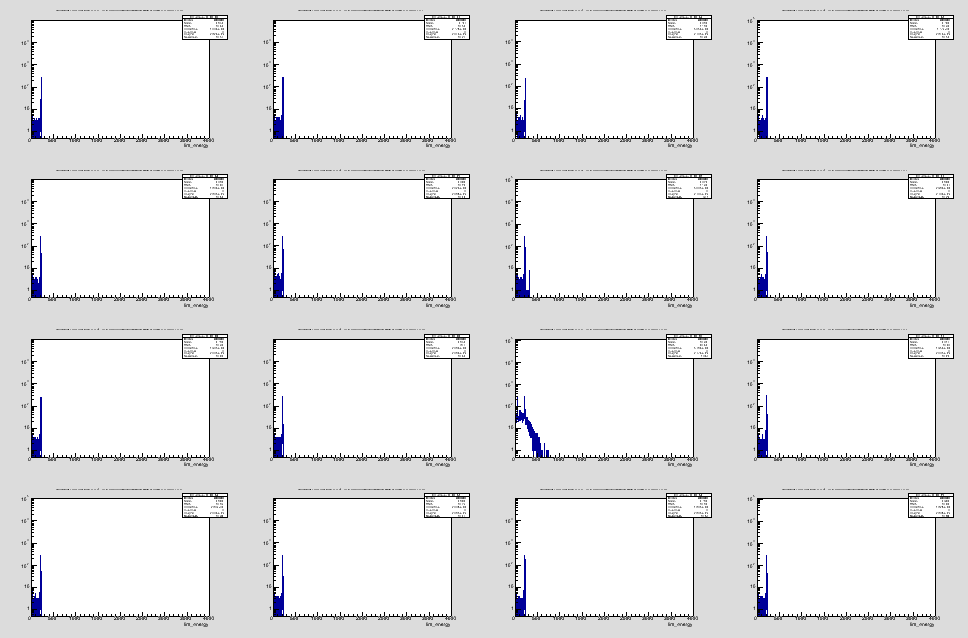
\includegraphics[width=\linewidth]{fopra_preamp_lim_energy_card1_all.png}
  \caption{FOPRA Preamp, card 1, all channels, no crystal, only pulser. Channel 10 noisy/broken.}
\end{figure}

\newpage
\clearpage
\subsection{Preamp 1}
To repair: All channels in both cards noisy.
\begin{figure}[!htb]
  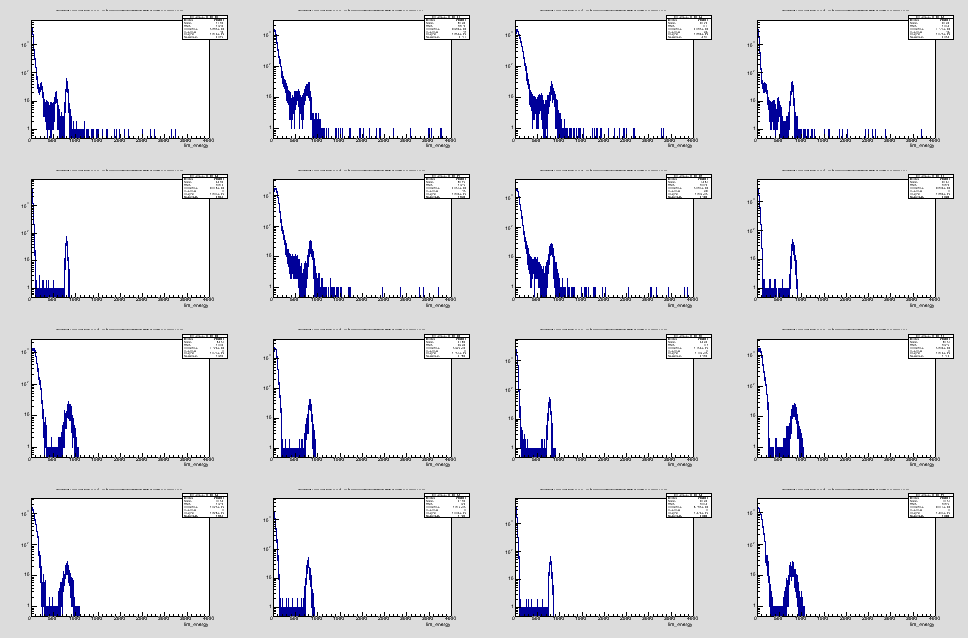
\includegraphics[width=\linewidth]{preamp1_lim_energy_card0_all.png}
  \caption{Preamp 1, card 0, all channels, Na22 source  with pulser. All channels noisy.}
\end{figure}

\begin{figure}[!htb]
  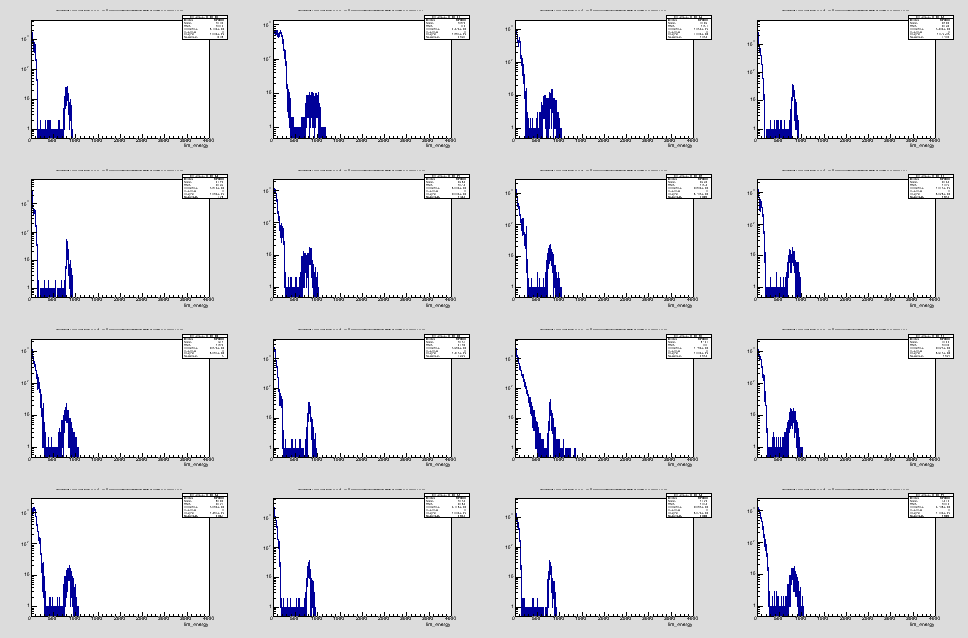
\includegraphics[width=\linewidth]{preamp1_lim_energy_card1_all.png}
  \caption{Preamp 1, card 1, all channels, no crystal, only pulser. All channels noisy.}
\end{figure}
\newpage
\clearpage

\subsection{Preamp 5}
To repair: missing channel 5 and 9.
\begin{figure}[!htb]
  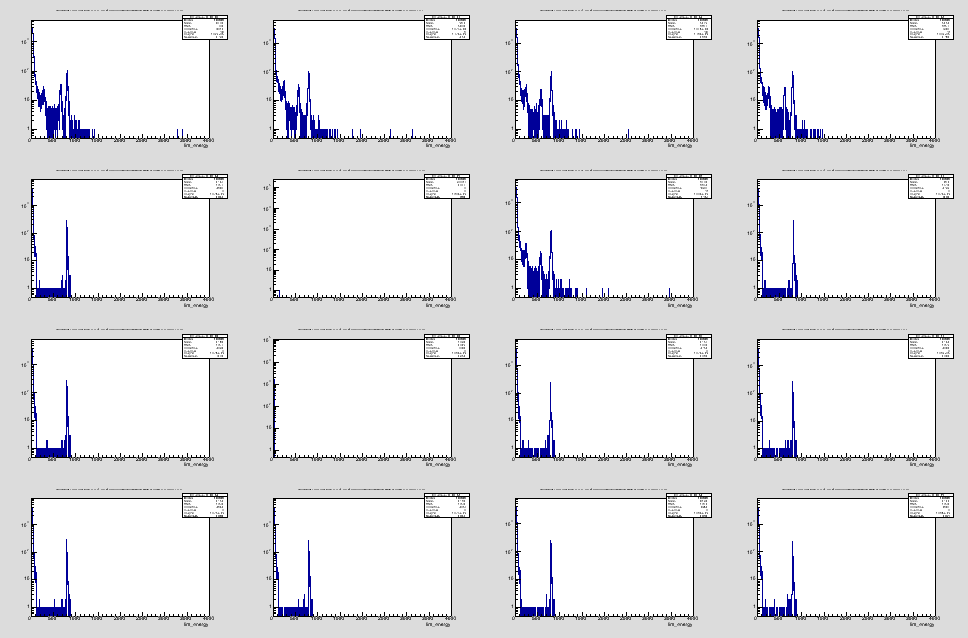
\includegraphics[width=\linewidth]{preamp5_lim_energy_card0_all.png}
  \caption{Preamp 5, card 0, all channels, Na22 source  with pulser. Missing channel 5 and 9.}
\end{figure}
\newpage
\clearpage




\subsection{Preamp 6 (Dual Range)}
To repair: card 0 channels 0,9,10,11,12,15 are noisy. card1 channels 7,8,9,10,11,12,15 are noisy.
\begin{figure}[!htb]
  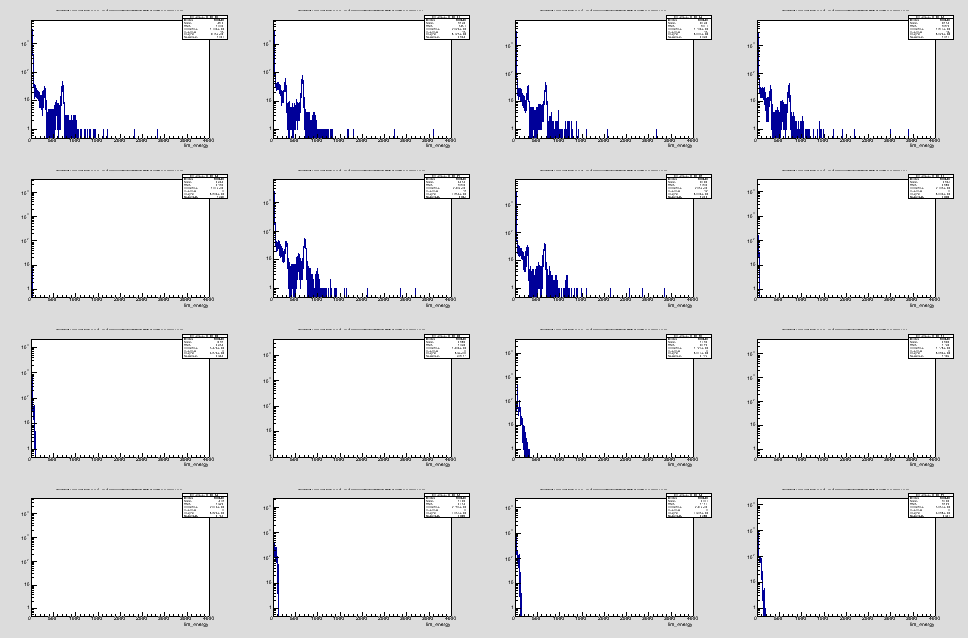
\includegraphics[width=\linewidth]{/dr_latest_test/preamp6_lim_energy_card0_all_no_pulser.png}
  \caption{Preamp 6, card 0, all channels, Na22 source  no pulser. Channels 0,9,10,11,12,15 are noisy }
\end{figure}

\begin{figure}[!htb]
  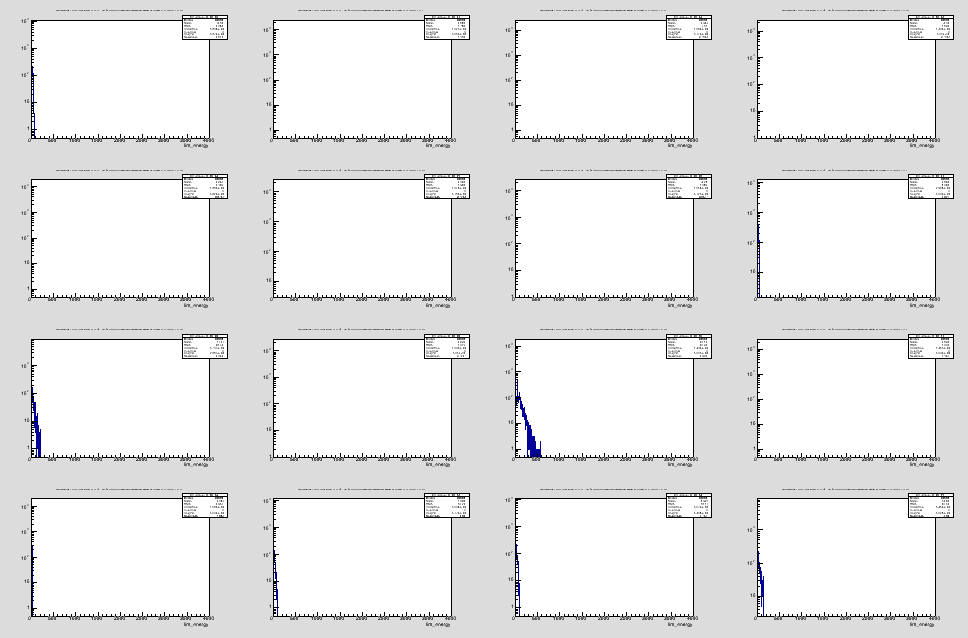
\includegraphics[width=\linewidth]{dr_latest_test/preamp6_lim_energy_card1_all_no_pulser.png}
  \caption{Preamp 6, card 1, all channels, Na22 source  no pulser. Channels 7,8,9,10,11,12,15 are noisy.}
\end{figure}
\newpage
\clearpage

\subsection{Preamp 7 (Dual Range)}
To repair: card 1 channels 0,7,8,10,13,14,15 are noisy.
\begin{figure}[!htb]
  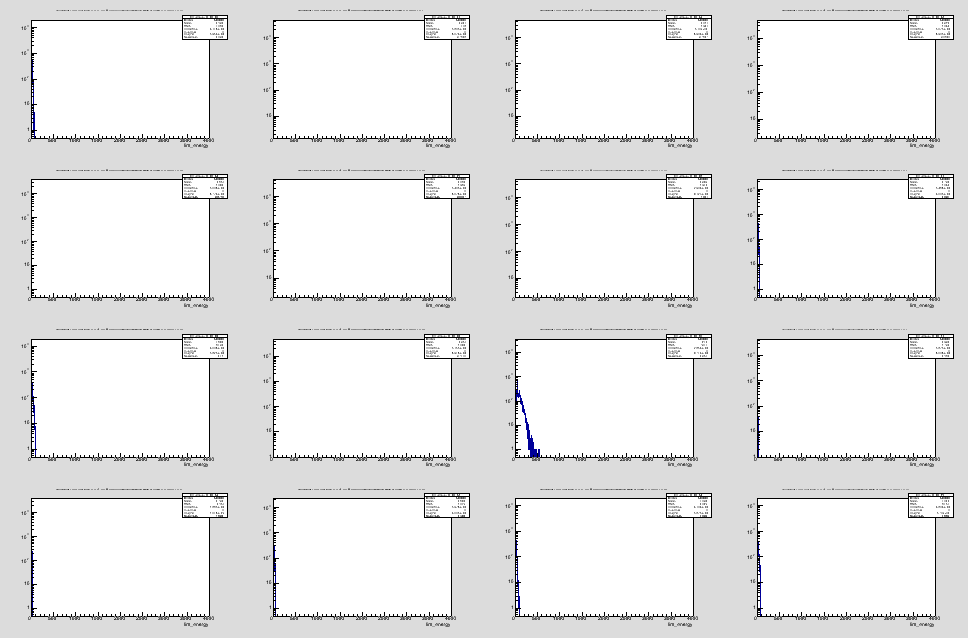
\includegraphics[width=\linewidth]{dr_latest_test/preamp7_lim_energy_card1_all_no_pulser.png}
  \caption{Preamp 7, card 1, all channels, Na22 source  no pulser. Channels 0,7,8,10,13,14,15 are noisy.}
\end{figure}

\newpage
\clearpage

\subsection{Preamp 8 (Dual Range)}
To repair: card 0 channels 8,9,10,11,12,15 are noisy. Card1 all channels are noisy.
\begin{figure}[!htb]
  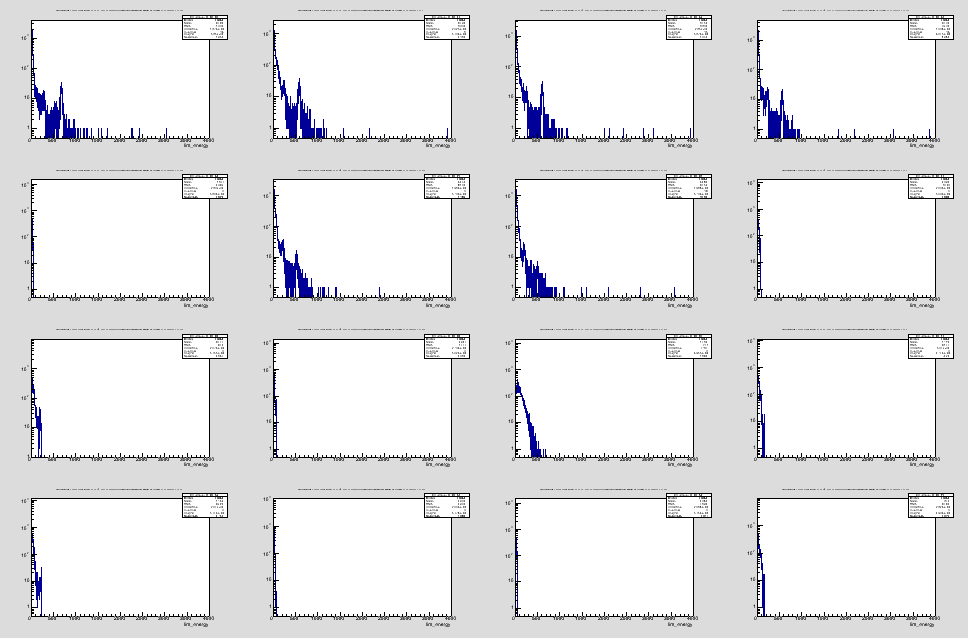
\includegraphics[width=\linewidth]{dr_latest_test/preamp8_lim_energy_card0_all_no_pulser.png}
  \caption{Preamp 8, card 0, all channels, Na22 source  no pulser. Channels 8,9,10,11,12,15 are noisy}
\end{figure}

\begin{figure}[!htb]
  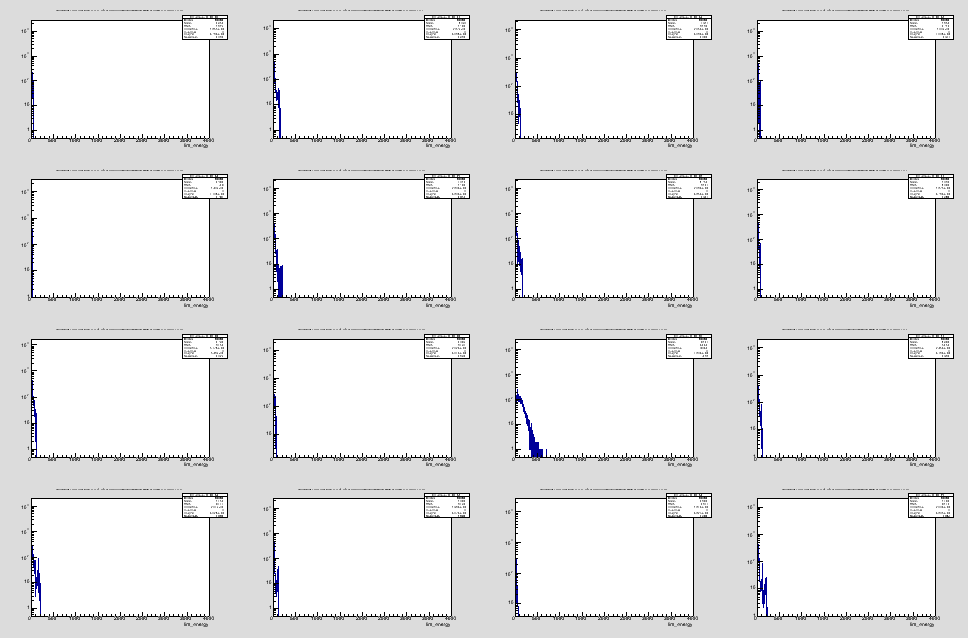
\includegraphics[width=\linewidth]{dr_latest_test/preamp8_lim_energy_card1_all_no_pulser.png}
  \caption{Preamp 8, card 1, all channels, Na22 source  no pulser. All channels are noisy.}
\end{figure}
\newpage
\clearpage


\subsection{Preamp 10}
To repair: card0 channels 10,11,15 are noisy.
\begin{figure}[!htb]
  \includegraphics[width=\linewidth]{small_box_card0_all_nopulser.png}
  \caption{Preamp 10, card 0, all channels, Na22 source  no pulser. Channels 10,11,15 are noisy.}
\end{figure}

\newpage
\clearpage

\section{Summary - repair demand}
Preamp 1, seems to be noisy in both cards (0,1), bad resolultion.\newline
Preamp 5, card 0: here we have missing channels 5 and 9.\newline
FOPRA Preamp, card 1: channel 10 noisy/broken.\newline
Preamp 6, card 0: 9,10,11,12,15 channels are noisy. card 1: 7,8,9,10,11,12,15 channels are noisy.\newline
Preamp 7, card 1: 0,7,8,10,13,14,15 channels are noisy\newline
Preamp 8, card0: 8,9,10,11,12,15 channels are noisy. card1: all channels noisy\newline
Preamp10,card 0: 10,11,15 channels noisy.\newline


\end{document}


